%------------------------------------------------------------------------------
%	CAPITOLO 5
%------------------------------------------------------------------------------

\chapter{Don Matteo G. e le sue prediche}
\index[Personaggi]{Don G. Matteo}Era un buon diavolo, senza istruzione, sacerdote di Cristo e... di Bacco, unico suo peccato.\\
\indent Fino alle 20,45 stava chiuso nella sua cantina a trincare di quel buon vino ... al quale aggiungeva dell'alcool, perché era troppo debole. Dalle 20,45 diventava astemio per preparasi col digiuno alla Santa Messa del mattino successivo. Non è da tacere che andava sempre a letto in garletta\footnote{Essere "in garlèta" di solito si dice di persona allegra, un po' sopra le righe, magari per qualche bicchiere di vino in più.} orando per forza d'abitudine. Celebrava continuamente la messa a San Francesco ed a Sant'Apollonia\footnote{\textbf{San Vincenzo} viene anche chiamata Santa Apollonia per il quadro dell'omonima santa che vi è all'interno. S. Vincenzo fu fabbricata circa il 1750 da Francesco de' conti Cervi Samaritani, famiglia venuta da Cremona nel 1509. Diventò un oratorio padronale di proprietà di Stefano Mingazzi. Oggi è di proprietà degli eredi di \index[Personaggi]{Minguzzi Egisto}Minguzzi Egisto, che comprò il terreno dai Ciechi di Bologna.} al \index[Luoghi]{Passetto}Passetto. Le popolazioni delle due strade gli volevano molto bene, ricorrevano a lui per gli annunzi dall'altare e subito lui li accontentava coi i seguenti pistolotti\footnote{Discorso ammonitorio ed esortativo} autentici:\\
\indent <<Popolo della \index[Luoghi]{Reale (via)}via Reale, è stato perduto un bottazzo\footnote{Direttamente spiegato dal Mingazzi nei suoi quaderni: "Per chi non lo sapesse, il bottazzo era un fustico, piccolo barile, di legno che i contadini portavano nel prato, in valle, col vino da bere durante i lavori"} pieno di vino; chi l'avesse ritrovato si beva il bottazzo e porti il vino...>> poi <<No, no am so sbaglié\footnote{<<No, no mi sono sbagliato>>} voglio dire si beva il vino e porti il bottazzo.>>\\
\indent Altro esempio:\\
\indent<<Popolo della \index[Luoghi]{Reale (via)}via Reale, è stata perduta una gabana\footnote{Termine dialettale per `giacca'} color di mezzalana\footnote{Don Matteo sbaglia l'associazione colore-materiale}, chi l'avesse ritrovata la porti...>>

I pistolotti suoi personali erano ancora più curiosi. \index[Personaggi]{Magrini}Magrini e altri ragazzi, gli disturbavano la messa, allora il buon prete semplicione, tralasciava le funzioni, si infiammava , e poi:\\
\indent <<Sa vègn fùra cun sta vinciastra a va més mè.\footnote{<<Se vengo fuori con questo vimine vi accomodo io>>}>>\\
\indent Le cose si quietavano per un po' poi i monelli ricominciavano ed il povero don Matteo\index[Personaggi]{Don G. Matteo} abbandonava la messa, pigliava il vimine e vestito dei sacri paramenti rincorreva i monelli per il cortile per picchiarli... I fedeli ridevano e compativano. 

La fine della sua officiatura\footnote{Celebrazione della funzione religiosa} a \index[Luoghi]{San Vincenzo `Sant'Appollonia'}S. Vincenzo fu proclamata da lui dall'altare, così:\\
\indent <<Popolo della via Reale\index[Luoghi]{Reale (via)} la Sgnora \index[Personaggi]{Lanconelli `Flipèna' Virginia}Flipèna (Lanconelli), l'è môrta, \index[Personaggi]{Samaritani Vittorio}Samartèn (allora padrone dell'oratorio) un'um pêga, e mè, la messa par gnint an la vèngn pui a dì\footnote{<<La Signora Filippina è morta, e Samaritani non mi paga, e io, la messa per niente non la vengo poi a dire>> - Si parla di \textbf{Samaritani Vittorio} e \textbf{Lanconelli Virginia}, detta Filippina.}>>\\
Con questa chiusa\footnote{Conclusione} cominciò la sua nuova officiatura al \index[Luoghi]{Passetto}Passetto. Colà i contadini andavano a messa con lo schioppo\footnote{Fucile}, del quale il nostro don Matteo\index[Personaggi]{Don G. Matteo} aveva un sacrosanto terrore. Allora uscì in uno dei suoi predicozzi:\\
\indent <<Popolo del \index[Luoghi]{Passetto}Passetto, vi proibisco di venire alla santa messa c'un che cazz che sbat, pet a cl'êtar, uv putrèb scapé una sciupté e amazé e povar zazardòt a l'altér cl'è inuzènt\footnote{<<...con quel cazzo che batte dirimpetto a quell'altro, vi potrebbe scappare una fucilata ad ammazzare il povero sacerdote, all'altare, che è innocente.>>}>>\\

Chiudiamo con un'ultima del semplicione. Funzionava da cappellano a \index[Luoghi]{Savarna}Savarna ed un giorno, verso sera, montato sul suo birroccino tirato dall'asino si prese da Alfonsine per tornare in parrocchia. Come il solito, aveva sul pomeriggio troppo brindato a Bacco e mal si reggeva in gambe. Nei pressi della \index[Luoghi]{Le Marianne}scoperta delle Marianne\footnote{La "Mariana" era una valle tra Alfonsine e \index[Luoghi]{Savarna}Savarna che venne bonificata e diventò una via che poi prese il nome di via \index[Luoghi]{Basilica (via)}Basilica. L'origine potrebbe derivare dai proprietari che erano i frati di \index[Luoghi]{Santa Maria in Porto}Santa Maria in Porto.}, sentì la necessità di una occorrenza... piantò l'asino della strada e si appiattì al di là di una siepe.

Quel che successe si deve indovinare; l'asino fu trovato alla mattina, coi finimenti, attaccato al biroccino, dietro la porte della stalla della Chiesa a \index[Luoghi]{Savarna}Savarna, ma del padrone nulla.

A mattino molto inoltrato, il prete si svegliò nel prato, dove era caduto per la solenne sbornia, perché il sole lo martellava... riandò agli avvenimenti della sera prima e nella mente un po' rischiarata, non trovando più l'asino... lo seguì a piedi... da buon soldato di Cristo.



 \begin{figure}[htb]
    \centering
    %\vspace{-0.7cm}
    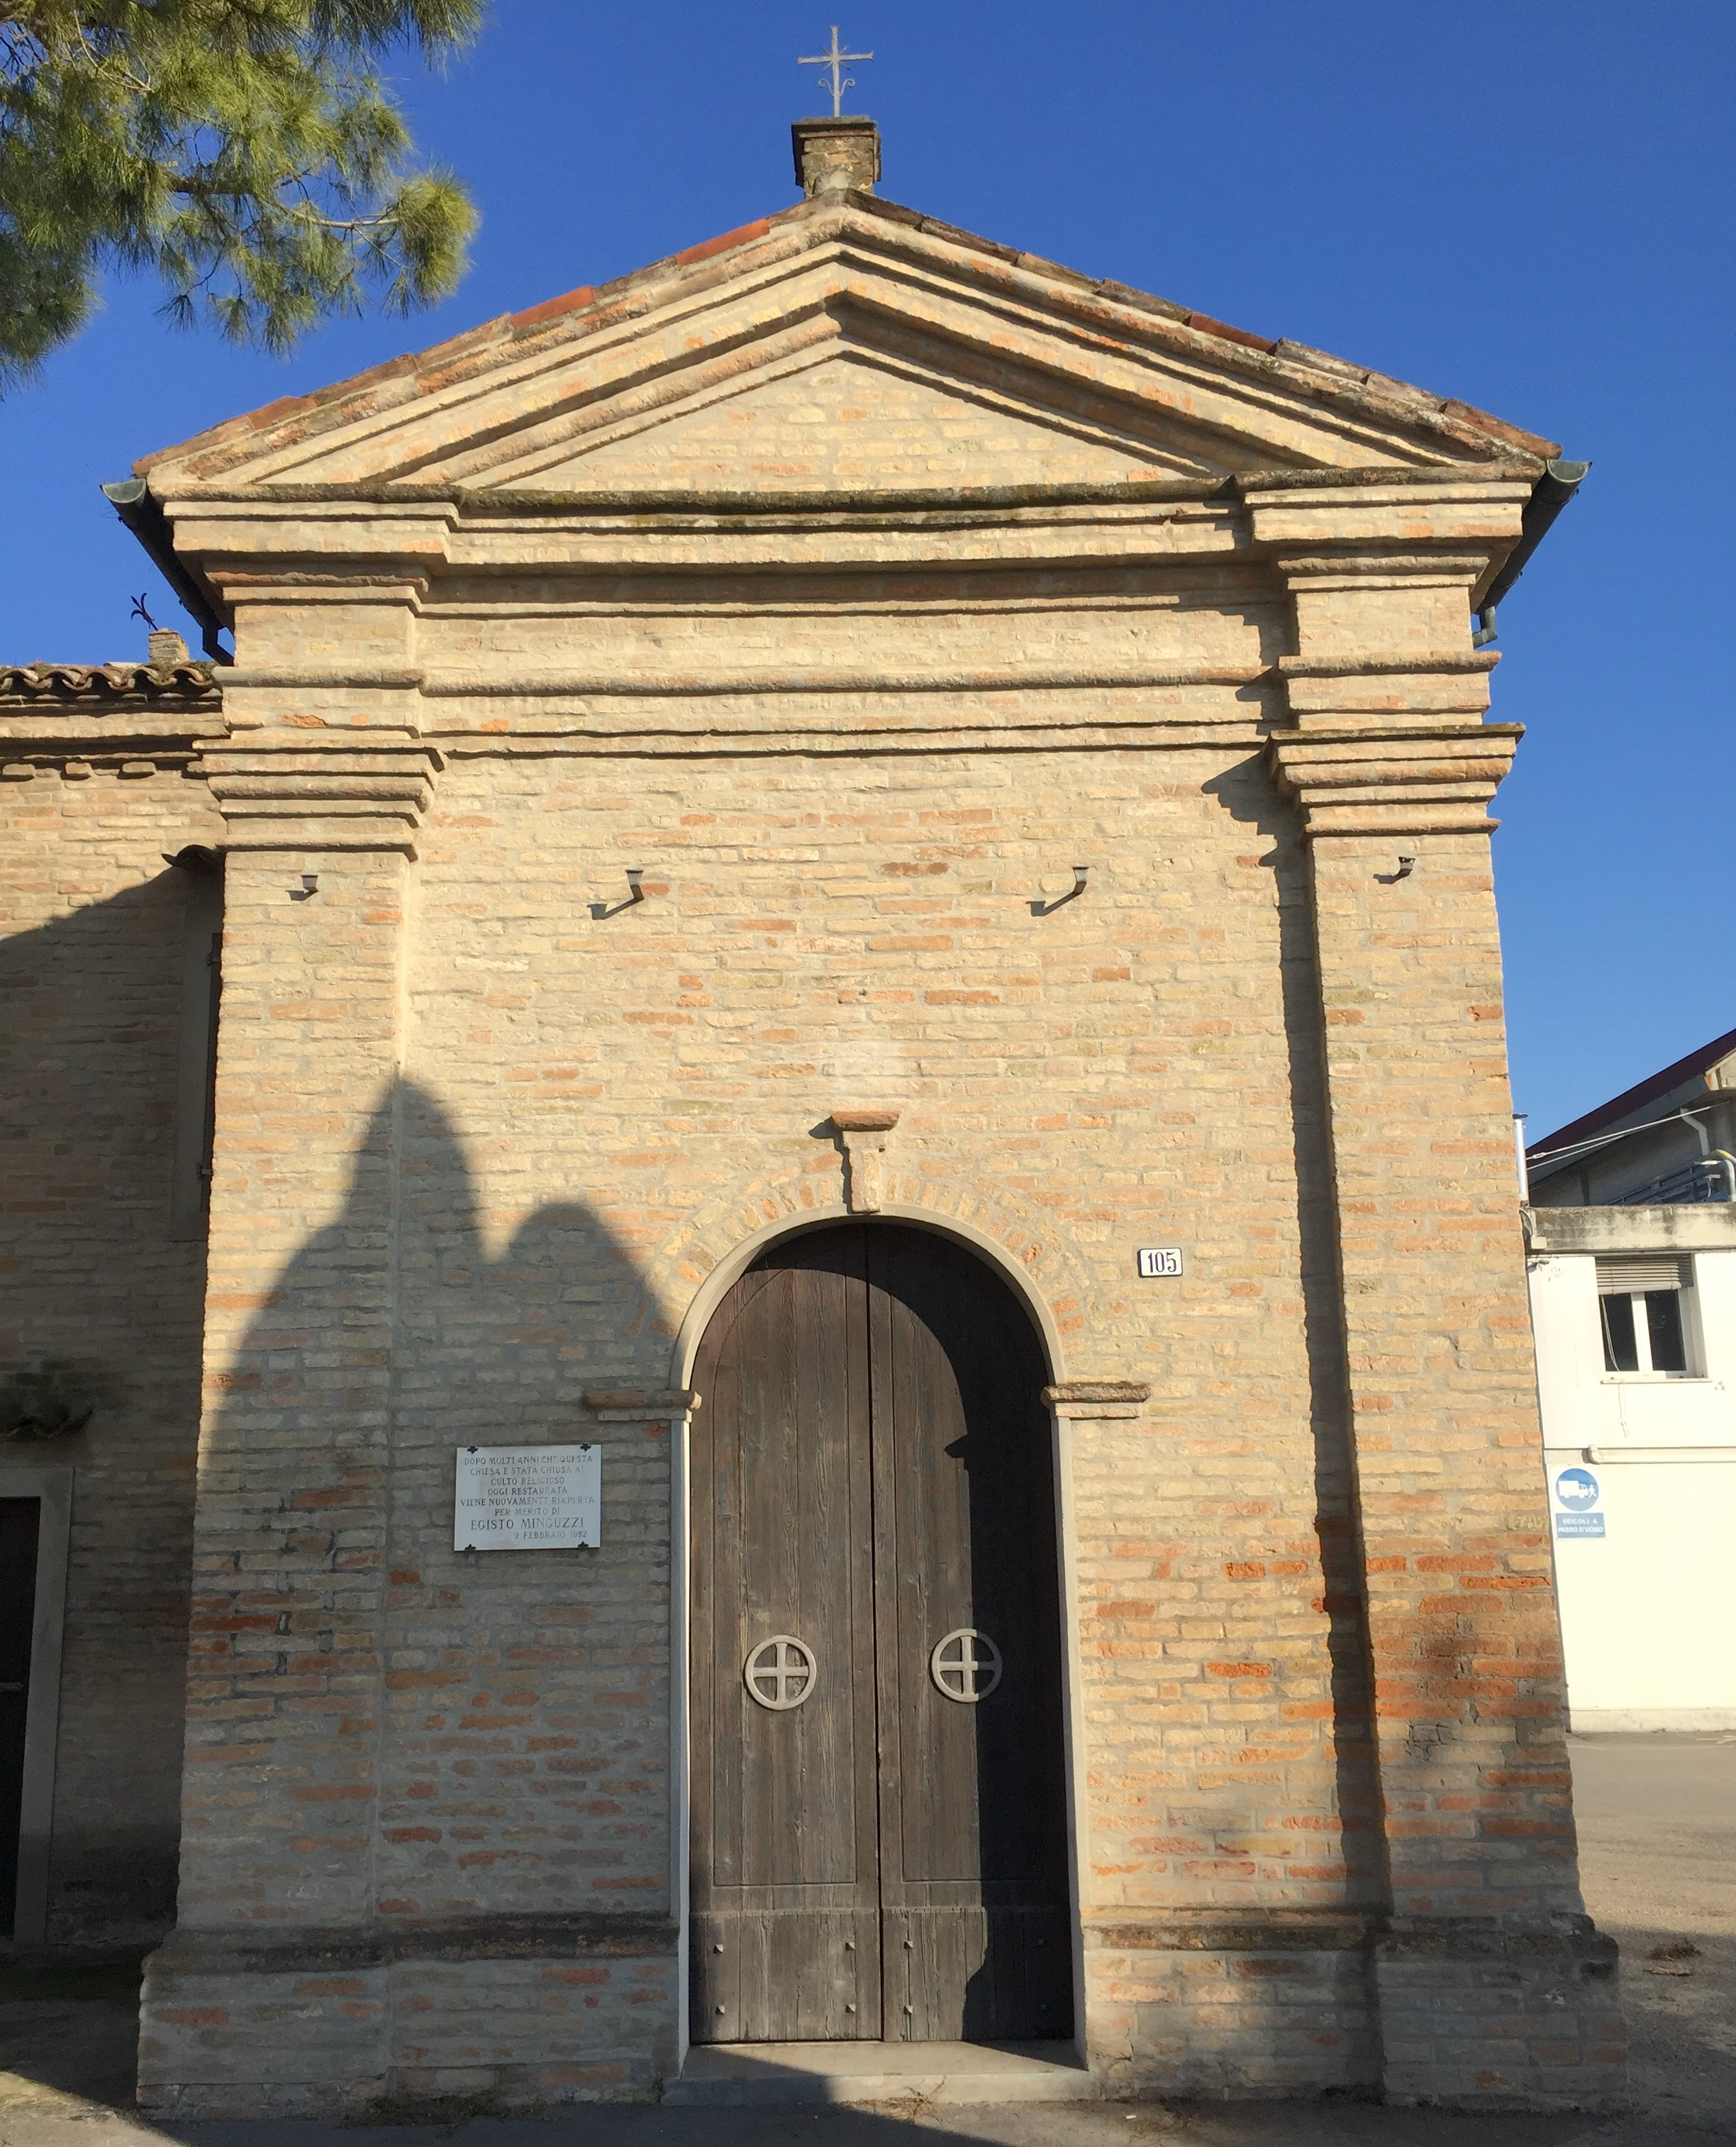
\includegraphics[width=\textwidth]{vincenzo}
    \caption*{\index[Luoghi]{San Vincenzo `Sant'Appollonia'}\textbf{San Vincenzo}, detta anche Sant'Apollonia. Nella targa vi è scritto:\\ "\textit{Dopo molti anni che questa chiesa è stata chiusa al culto religioso, oggi restaurata, viene nuovamente riaperta per merito di Egisto Minguzzi, 9 febbraio 1982}"\label{fig:vincenzo}}
    %\vspace{-0.3cm}
\end{figure}










































%

